%  LaTeX support: latex@mdpi.com
%  For support, please attach all files needed for compiling as well as the log file, and specify your operating system, LaTeX version, and LaTeX editor.

%=================================================================
\documentclass[remotesensing,article,submit,pdftex,moreauthors]{Definitions/mdpi}

%=================================================================
% MDPI internal commands - do not modify
\firstpage{1}
\makeatletter
\setcounter{page}{\@firstpage}
\makeatother
\pubvolume{1}
\issuenum{1}
\articlenumber{0}
\pubyear{2024}
\copyrightyear{2024}
%\externaleditor{Academic Editor: Firstname Lastname}
\datereceived{ }
\daterevised{ } % Comment out if no revised date
\dateaccepted{ }
\datepublished{ }
%\datecorrected{} % For corrected papers: "Corrected: XXX" date in the original paper.
%\dateretracted{} % For corrected papers: "Retracted: XXX" date in the original paper.
\hreflink{https://doi.org/} % If needed use \linebreak
%\doinum{}
%\pdfoutput=1 % Uncommented for upload to arXiv.org
%\CorrStatement{yes}  % For updates


%=================================================================
% Add packages and commands here. The following packages are loaded in our class file: fontenc, inputenc, calc, indentfirst, fancyhdr, graphicx, epstopdf, lastpage, ifthen, float, amsmath, amssymb, lineno, setspace, enumitem, mathpazo, booktabs, titlesec, etoolbox, tabto, xcolor, colortbl, soul, multirow, microtype, tikz, totcount, changepage, attrib, upgreek, array, tabularx, pbox, ragged2e, tocloft, marginnote, marginfix, enotez, amsthm, natbib, hyperref, cleveref, scrextend, url, geometry, newfloat, caption, draftwatermark, seqsplit
% cleveref: load \crefname definitions after \begin{document}

%=================================================================
% Please use the following mathematics environments: Theorem, Lemma, Corollary, Proposition, Characterization, Property, Problem, Example, ExamplesandDefinitions, Hypothesis, Remark, Definition, Notation, Assumption
%% For proofs, please use the proof environment (the amsthm package is loaded by the MDPI class).

%=================================================================
% Full title of the paper (Capitalized)
\Title{Robot Team III: Scotty Strikes Back}

% MDPI internal command: Title for citation in the left column
\TitleCitation{Title}

% Author Orchid ID: enter ID or remove command
\newcommand{\orcidauthorA}{0000-0002-5910-0183} % John
\newcommand{\orcidauthorB}{0000-0003-2688-648X} % Lakitha
\newcommand{\orcidauthorC}{0000-0002-9841-6703} % Shawhin
\newcommand{\orcidauthorD}{0000-0003-2657-3416} % Prabuddha
\newcommand{\orcidauthorE}{0000-0003-4265-9543} % David
\newcommand{\orcidauthorF}{0000-0003-0667-2345} % Ash
\newcommand{\orcidauthorG}{0000-0002-0126-218X} % Adam
% \newcommand{\orcidauthorH}{} % Gokul

% Authors, for the paper (add full first names)
\Author{John Waczak \orcidA{}, Adam Aker \orcidG{}, Lakitha O. H. Wijeratne \orcidB{}, Shawhin Talebi \orcidC{}, Ashen Fernando \orcidF{}, Prabuddha M. H. Dewage \orcidD{}, Mazhar Iqbal, Matthew Lary, David Schaefer, Gokul Balagopal, and David J. Lary *\orcidE{}}

%\longauthorlist{yes}

% MDPI internal command: Authors, for metadata in PDF
\AuthorNames{John Waczak, Adam Aker, Lakitha O. H. Wijeratne, Shawhin Talebi, Bharana Fernando, Prabuddha Hathurusinghe, Mazhar Iqbal, Matthew Lary, David Schaefer, Gokul Balagopal, and David J. Lary}

% MDPI internal command: Authors, for citation in the left column
 \AuthorCitation{Waczak, J.; Aker, A.; Wijeratne, L.O.H.; Talebi, S.; Fernando, B.; Hathurusinghe, P.; Iqbal, M.; Lary, M.; Schaefer, Balagopal, G.; D.; Lary, D.J.}
% If this is a Chicago style journal: Lastname, Firstname, Firstname Lastname, and Firstname Lastname.

% Affiliations / Addresses (Add [1] after \address if there is only one affiliation.)
\address[1]{%
Hanson Center for Space Sciences, University of Texas at Dallas, Richardson, TX 75080, USA;  john.waczak@utdallas.edu (J.W.); adam.aker@utdallas.edu (A.A.); lhw150030@utdallas.edu (L.O.H.W.); shawhintalebi@gmail.com (S.T.); ashen.fernando@utdallas.edu  (B.F.); pxh180012@utdallas.edu (P.M.H.D.); mazhar.iqbal@utdallas.edu (M.I.); MDL210001@utdallas.edu (M.L.); captdaveschaefer@gmail.com (D.S.); gokul.balagopal@utdallas.edu (G.B.);}

% Contact information of the corresponding author
\corres{Correspondence: david.lary@utdallas.edu} %; Tel.: (optional; include country code; if there are multiple corresponding authors, add author initials) +xx-xxxx-xxx-xxxx (F.L.)}


% Abstract (Do not insert blank lines, i.e. \\) 
\abstract{
Unmanned Aerial Vehicles (UAVs) equipped with hyperspectral imagers have emerged as a pivotal technology for the characterization of inland water bodies. The high spectral and spatial resolutions of these systems enable the retrieval of a plethora of optically-active water quality parameters via band ratio algorithms and machine learning methods. However, fitting and validating these models requires access to sufficient quantities of in situ reference data which are time-consuming and expensive to obtain. 
In this study, we demonstrate how the Generative Topographic Mapping (GTM), a Bayesian realisation of the Self Organizing Map (SOM), can be effectively used to enable unsupervised classification and nonlinear endmember extraction of UAV acquired hyperspectral imagery. Using imagery collected across a North Texas Pond, we demonstrate how th
- to enable fully unsupervised classification UAV acquired hyperspectral imagery.
-The methods is fully Bayesian, providing an attractive method for the unsupervised classification of hyperspectral imagery. 
- generative topographic mapping (GTM) as an efficient unsupervised method 
- additionally the GTM can be used to perform nonlinear endmember extraction
- We demonstrate the abilities of this approach using hyperspectral imagery collected at a pond in Montague, North Texas.
- First, we apply the GTM to perform an unsupervised classification for all water pixels. 
    - benefit: GTM classes maintain topological relationships in the latent space resulting in a smooth relationship between the obtained classes...
    - ... revealing the small-scale spatial variability within the pond
- Second, we utilize the GTM to identify reflectance spectra corresponding to specific features. 
- Using these extracted features, we are able to map the extent of algae in the pond in addition to the time evolution of a rhodamine dye tracer. 
- This approach demonstrates the value of unsupervised techniques coupled with UAV-born hyperspectral imaging for rapid water quality assessment.
}

% Keywords
\keyword{Hyperspectral Imaging; Remote Sensing; Unsupervised Classification; Endmember Extraction, Spectral Unmixing} 


%%%%%%%%%%%%%%%%%%%%%%%%%%%%%%%%%%%%%%%%%%
\begin{document}

%%%%%%%%%%%%%%%%%%%%%%%%%%%%%%%%%%%%%%%%%%
\section{Introduction}


Inland water bodies pose a unique challenge for analysis with remote sensing imagery due to their complex spectral characteristics and small-scale spatial variability. Nevertheless, significant effort has driven the development of techniques for estimating optically-active water quality parameters such as chlorophyll-a, blue-green algae, colored dissolved organic matter (CDOM), turbidity, and temperature from these sources\cite{koponen2002lake,ritchie2003remote, bonansea2015using}. Machine learning has proven to be a powerful tool in this domain, with tree-based models, support vector machines, deep neural networks, and others architectures providing data-driven approaches mapping imagery to parameters of interest \cite{thenkabail2018hyperspectral, ghatkar2019classification,sagan2020monitoring}. However, the training and evaluation of these models demands significant volumes of coincident, in situ data. Collecting these datasets is time consuming and expensive, often requiring observations spanning decades \cite{aurin2018remote, ross2019aquasat}. 

To support and enhance real-time decision making, data-driven techniques...


The characterization of inland water bodies by remote sensing imagery poses a distinct challenge due to their complex spectral characteristics and small-scale spatial variability \cite{ritchie2003remote}. Traditional multi-spectral imagers utilized by these sensing platforms have large pixel sizes, limited spectral bands, and long revisit times.
- Nevertheless, ... 
- Machine learning has proven... 
- However, these techniques demand significant volumes of in situ data...
- To address the 

Hyperspectral imaging
- Hyperspectral imaging has emerged as a pivotal technology in this space.
- With their increased spectral resolution, hyperspectral imagers (HSIs) capture the complex chemical, biological, environmental characteristics of reflectance spectra. (add references for specific applications of HSIs). 
- However HSIs alone do not address the limited spatial resolution of 


UAV
- Advancements in hyperspectral imaging technology have lead to a continual decrease in their size facilitating their inclusion as the payload of small, highly maneuverable unmanned aerial vehicles (UAVs) such as drones. Consequently, much work has gone into the development of UAV platforms and associated techniques 
- Near-earth HSI addresses spatial, spectral, and temporal limitations of satellite and airborne platforms. UAV-based HSI enable fine-scale mapping \cite{banerjee2020uav}
- Drones can be equipped with HSI and compute to enable rapid generation of spectral indices like the NDVI for applications such as precision agriculture \cite{horstrand2019uav}
- UAV-based HSI can be georectified to centimeter-scales without need for ground control points by using on-board GPS and IMU \cite{arroyo2019implementation}
- UAV-based HSI for turbidity estimation \cite{vogt2016near}
- Polynomial regression models for chlorophyll-a, turbidity \cite{zhang2022selection}
- For this to be usefull, we still need the in situ data. By combining a UAV born HSI with simultanous collection of ground truth data by a reference sensor equipped autonomous boat, we are able to rapidly train ML models to 


Unsupervised Methods
- classic unsupervised ML
- endmember extraction and spectral unmixing

This paper...
- our approach is to use the GTM (a fully Bayesian realization of the self organizing map developed by Biship et al.)
- We demonstrate the capabilities using hyperspectral imagery collected at pond in Montague, North Texas. 
- First we utilize the GTM to perform an unsupervised classification of the water-only pixels in order to reveal the centimeter-scale structures present in the pond
- Next we showhow the GTM can be used to identify relevent spectral endmembers by 
    1. using learned GTM class signatures to identity the abundance of algae (relevant for Harmful Algal Bloom detection)
    2. use the GTM class signatures to map the evolution of a rhodamine tracer dye plume







 
- \cite{koponen2002lake}
- Example: distinguishing species for harmful algal blooms (HABs) and distinguishing types of oil for oil spill monitoring
- Remote sensing used for oil spill analysis: extent and thickness mapping \cite{kokaly2013spectroscopic, leifer2012state}

- Sun glitter remains a key challenge for sensing in the visible portion of the spectrum but multi and hyperspectral imagers have been used for oil spill identification and to identify their impacts on vegetation stress and mortality \cite{fingas2014review, khan2018modern}


Continued development of HSI technology has led to a dramatic reduction in their size enabling their utilize as the payload of small autonomous aerial vehicles (UAVs) (citation). By flying close to the ground UAV-born hyperspectral imagers can produce centimeter-scale imagery while simulatenously limiting the need for complicated atmospheric corrections required for satellite platforms (citation).

- applications include food quality & safety, medical diagnoses, precision agriculture, and forensic document examination \cite{khan2018modern}
- Hyperspectral data were used to distinguish oils by type, e.g. crude, diesel, gasoline, and palm \cite{yang2020characterization}


Unsupervised classification
- When no ground-truth data are available, unsupervised classification can still help partition imagery into groups or clusters.
- Many data-driven, ML methods have been employed for the task including various matrix factorizations, k-nearest neighbors, fuzzy c-means, density estimation methods, etc. \cite{zhang2019hyperspectral}
- Additionally unsupervised approaches can be used to perform nonlinear dimensionality reduction & pre-processing for supervised approaches.
- Many unsupervised approaches can be challenging to interpret due to the lack of a relationship between the identified classes, e.g. is class 1 more similar to class 2 than class 10?
- The Self Organizing Map is a popular technique which classifies data while enforcing topological relationships between the resulting classes such that classes close to each  other in the latent space are more similar than classes that are far apart.
- SOM used for remote sensing imagery classification \cite{msom-remote-sensing}
- SOM used for clustering and data compression of HSI cube-sat \cite{danielsen2021self}
- SOM used for land-use and land-cover change analysis \cite{penfound2021analysis}
- SOM has bee nused for identifying synoptic-scale patterns in wind and sea surface temperature data {som-satellite}


endmember extraction, spectral unmixing
- This is a related problem where the goal is to identify unique spectral signatures which combine (linearly or non-linearly) to produce the measured signal.
- Having identified the set of endmembers, we then seek to determine their relative abundance in each pixel
- Many statistical approaches for extracting endmembers \cite{berman2004ice}
- Sparse PCA used for endmember extraction \cite{yousefi2016mineral}
- Popular spectral unmixing approach is to treat "pure" endmembers as vertices of a simplex \cite{plaza2012endmember, nascimento2005vertex}
- Convolutional Neural Networks with Autoencoder architectures are a popular ML approach which identify endmembers and perform non-linear unmixing \cite{palsson2020convolutional, non-negative-autoencoders, su2019daen, borsoi2019deep}
- Self Organizing Map is another approach which has been used for endmember extraction together with neural networks for abundance mapping (unmixing) \cite{cantero2004analysis}



In our previous work, we introduced a robot team designed to rapidly characterize water composition in novel environments \cite{robot-team-1}. 
Joining UAV-borne HSI together with collection of in-situ reference data by an autonomous boat dramatically reduces the time required to generate .

By carefully coordinating the simultanous collection of ground-truth water quality data and hyperspectral imagery, this team can rapidly estimate concentrations of optically-active components including colored dissolved organic matter (CDOM), blue-green algae, crude oil, temperature as well 


In this paper, we demonstrate how Generative Topographic Mapping (GTM), a Bayesian alternative to the Self Organizing Map, can be utilized to rapidly identify relevant spectral signatures within a scene.

Using data collected at site in Montague, North Texas, we demonstrate the ability of this paradigm with two case studies. First, we demonstrate how the GTM can be used to provide a high-resolution unsupervised classification of a water body enabling the rapid identification of relevant regions which can then be used to direct further investigation by reference-sensor equipped boats. Second, we demonstrate the ability to perform endmember extraction and abundance mapping using imagery from a test-release of rhodamine dye. Together with the normalized spectral similarity score, these spectral signatures are identified and their associated area in the scene is determined.


In this study, we demonstrate how Generative Topographic Mapping (GTM), a Bayesian extension the Self Organizing Map, can be utilized to 



%%%%%%%%%%%%%%%%%%%%%%%%%%%%%%%%%%%%%%%%%%
\section{Materials and Methods}

\begin{figure}[t]
%\begin{adjustwidth}{-\extralength}{0cm}
\centering
%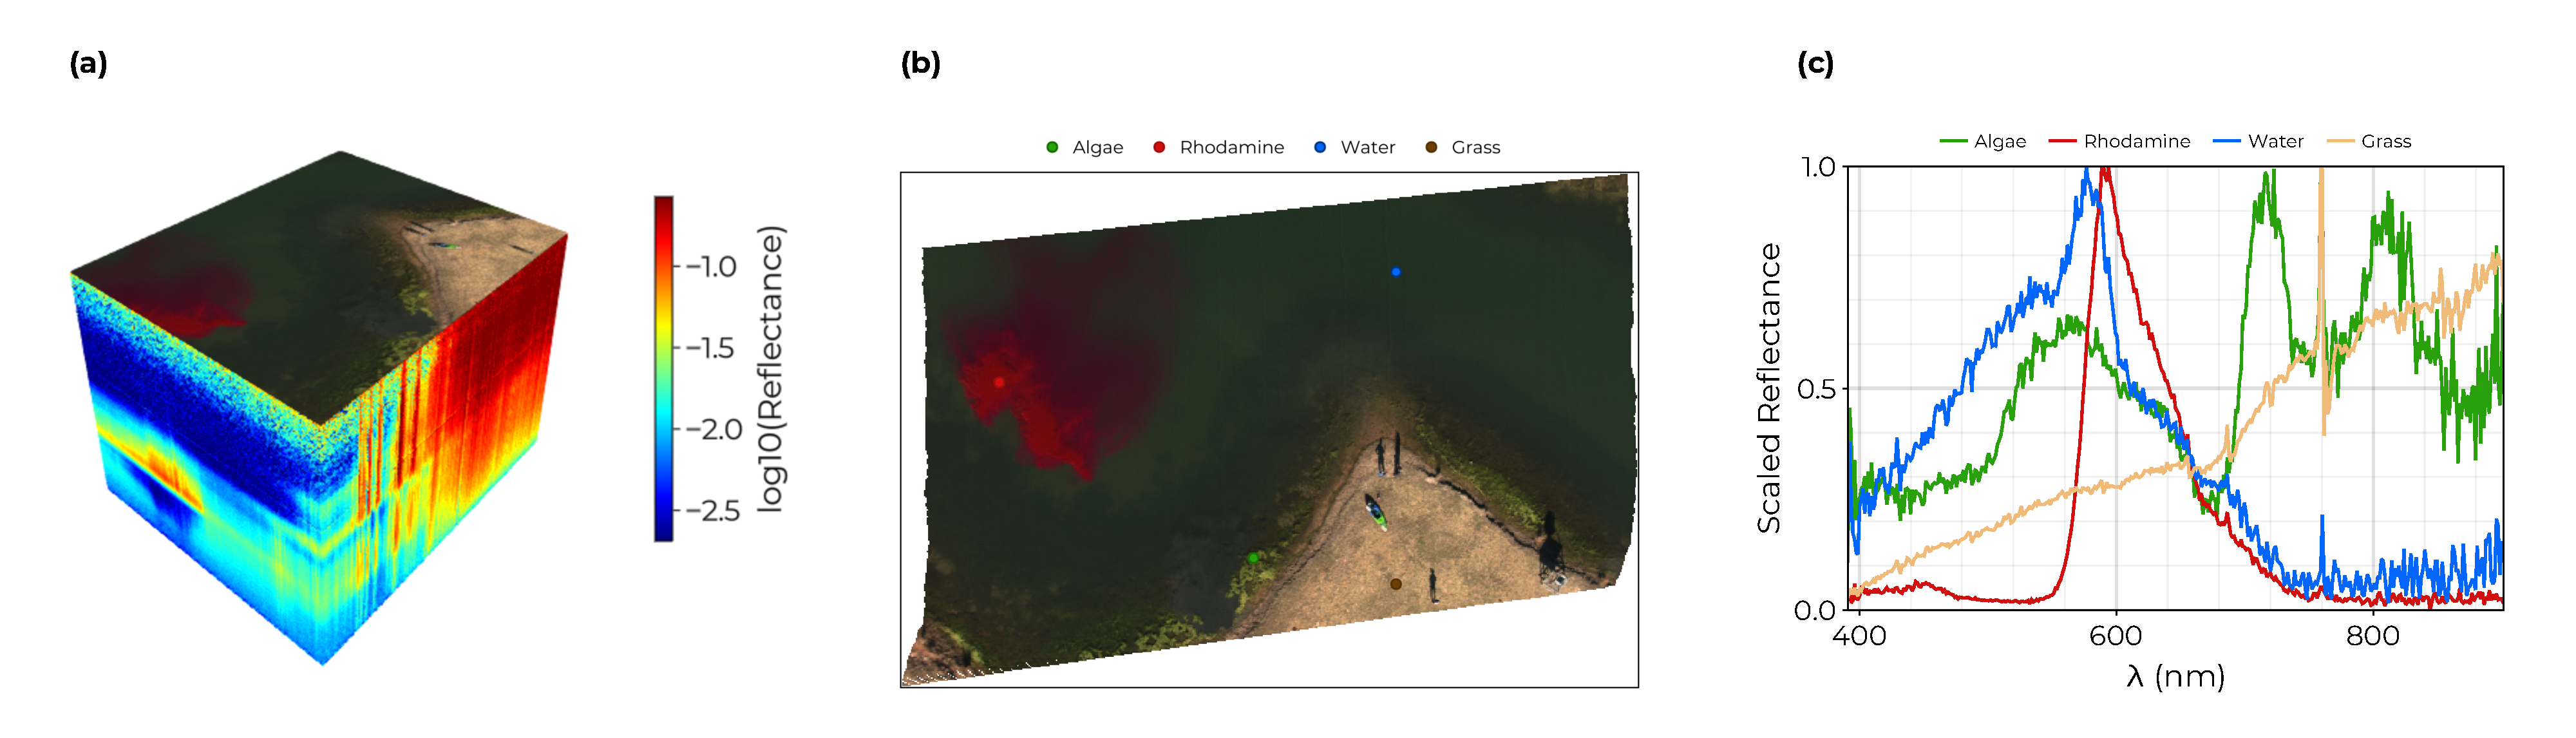
\includegraphics[width=15.5cm]{paper/figures/methods/sample-spectra.pdf}
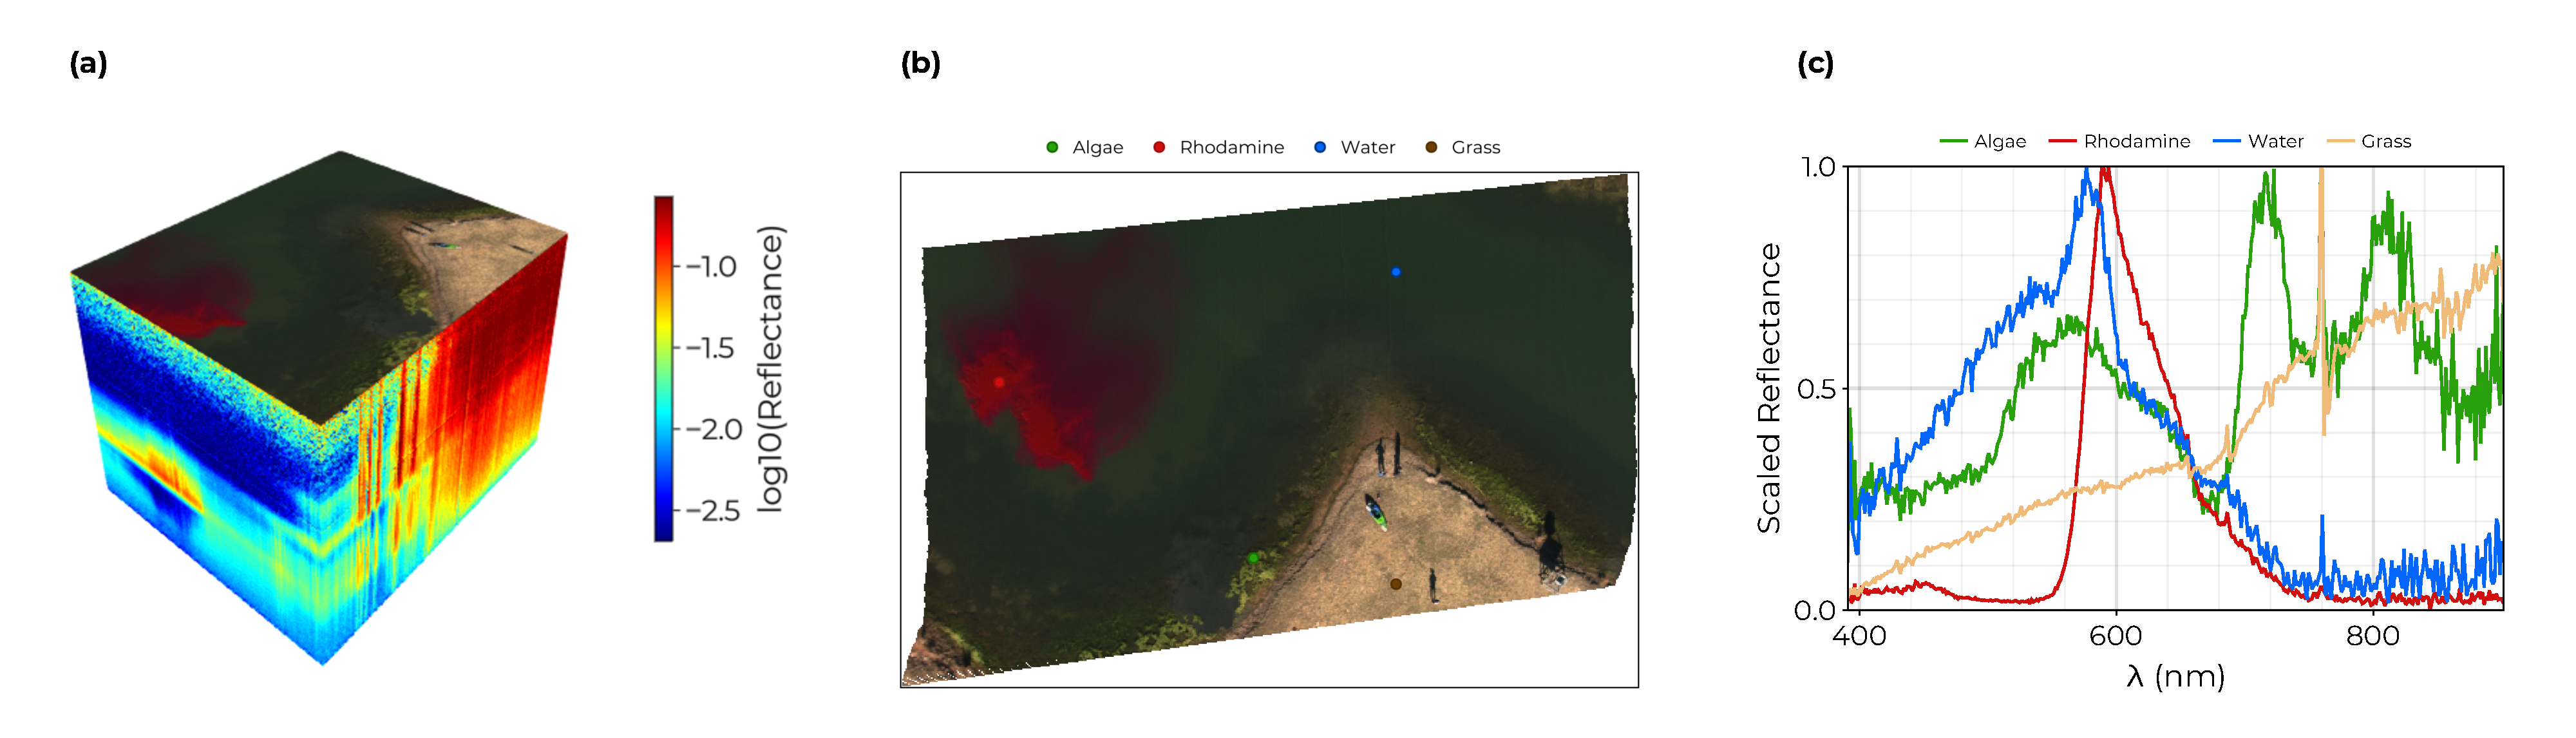
\includegraphics[width=\columnwidth]{paper/figures/methods/sample-spectra.pdf}
%\end{adjustwidth}
\caption{(a) Sample hyperspectral data cube. Spectra are plotted using their geographic position with the log10-reflectance colored along the z axis and a pseudo-color image on top. (b) Points taken from a sample hyperspectral data cube corresponding to algae, rhodamine dye, water, and dry grass. (c) The associated spectra for the exemplar points scaled so that the peak value of each spectrum is 1. (d) The location of the pond in Montague, Texas where data were collected for this study.\label{fig:sample-spectra}}
\end{figure}  


\subsection{Autonomous Robot Team}
\subsection{Data Collection and Pre-Processing}

- georetification \cite{muller2002program, baumker2001new, mostafa2000multi}

- Julia programming language used \cite{bezanson2012julia}

\subsection{Generative Topographic Mapping}

- GTM paper oricinal \cite{gtm-bishop-1}
- GTM developments paper \cite{gtm-biship-2}

- implementation designed to work in MLJ ecosystem \cite{blaom2020mlj}


\subsection{Image Segmentation with the Normalized Spectral Similarity Score}

%%%%%%%%%%%%%%%%%%%%%%%%%%%%%%%%%%%%%%%%%%
\section{Results}

\subsection{GTM Fit}

\begin{figure}[t]
\centering
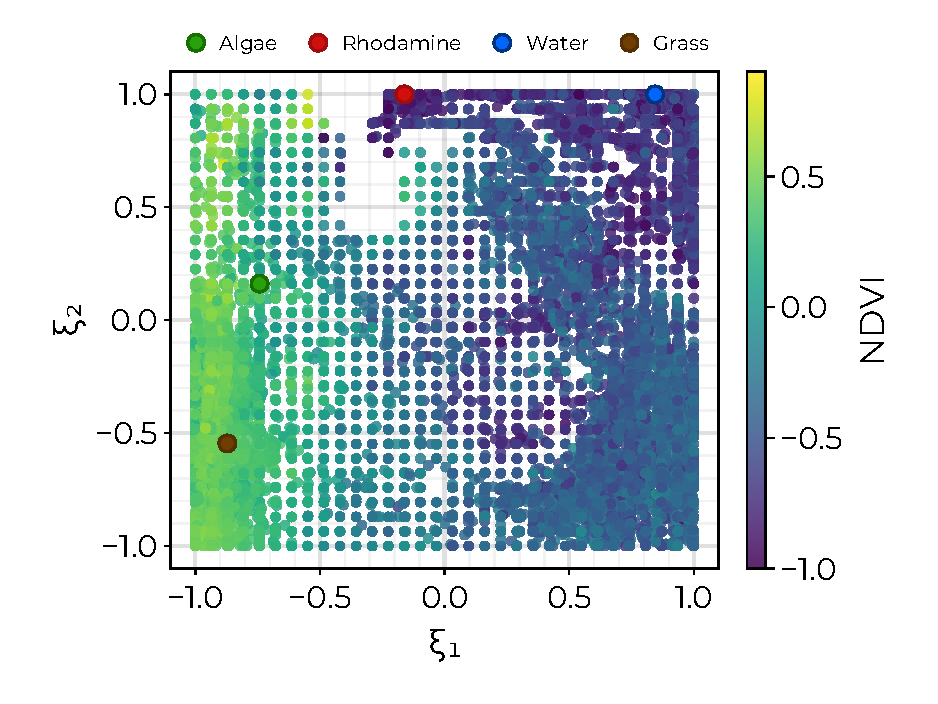
\includegraphics[width=0.8\columnwidth]{paper/figures/results/square-ndvi.pdf}
\caption{GTM Map: We plot the mean position of each data point in the latent space with points colored by the their associated NDVI values. The locations of the exemplar points for algae, rhodamine dye, water, and dry grass are shown in the latent space illustrating that the GTM has clearly distinguished land, near-land, and water pixels.\label{fig:}}
\end{figure}  


\subsection{Hyperparamter Optimization with BIC}


\begin{figure}[t]
%\begin{adjustwidth}{-\extralength}{0cm}
\centering
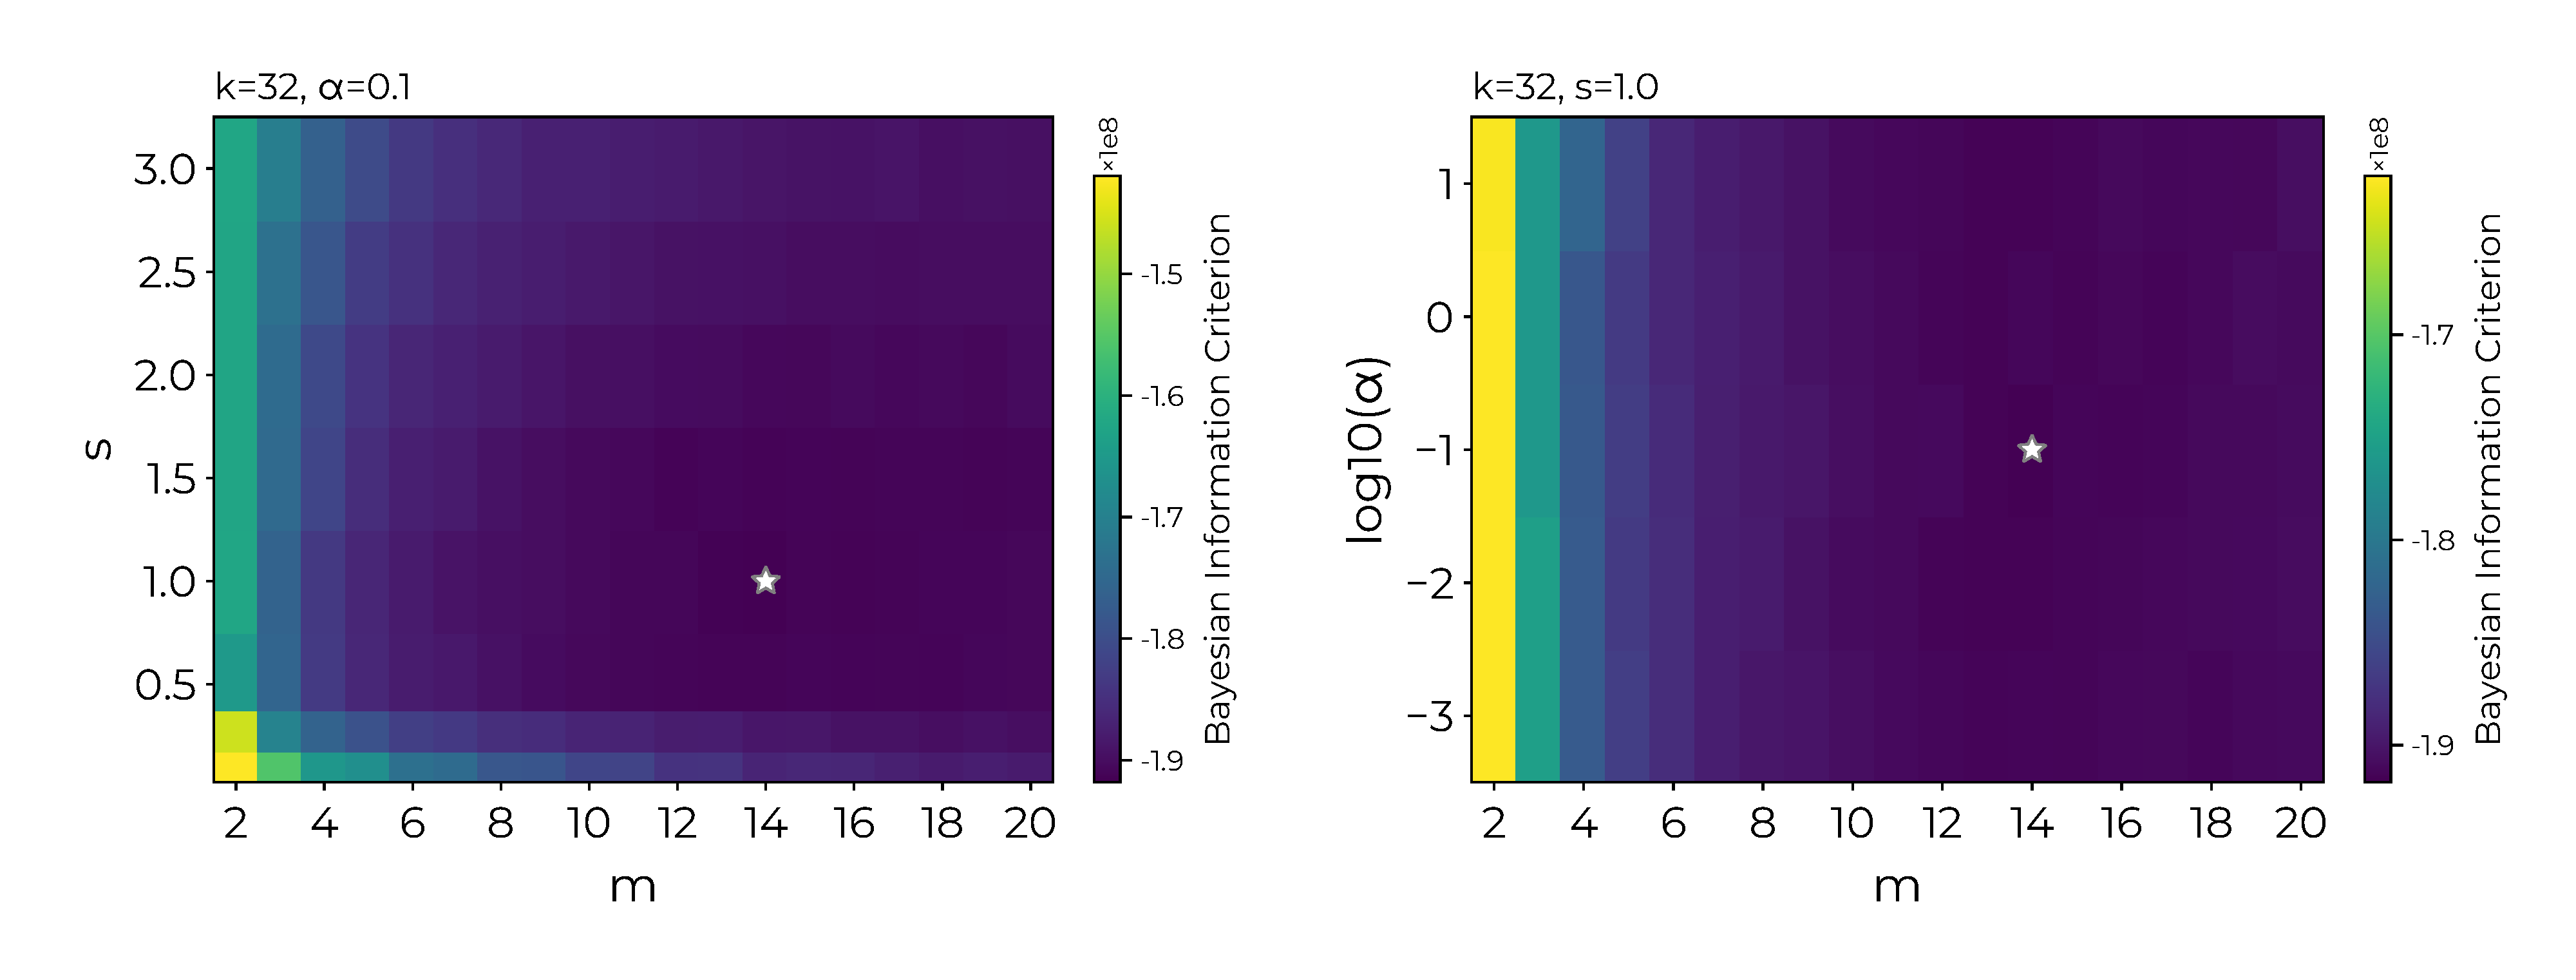
\includegraphics[width=\textwidth]{paper/figures/results/bic.pdf}
%\end{adjustwidth}
\caption{Results of the hyperparameter search. Left: Variation of BIC with $m$ and $s$ for fixed $\alpha=0.1$. Right: Variation of the BIC with with $m$ and $\alpha$ for fixed $s=1.0$. The white star in each plot indicates the parameters with the lowest BIC.\label{fig:hp-results}}
\end{figure}  


\subsection{Spectral Signatures}


\begin{figure}[t]
\begin{adjustwidth}{-\extralength}{0cm}
\centering
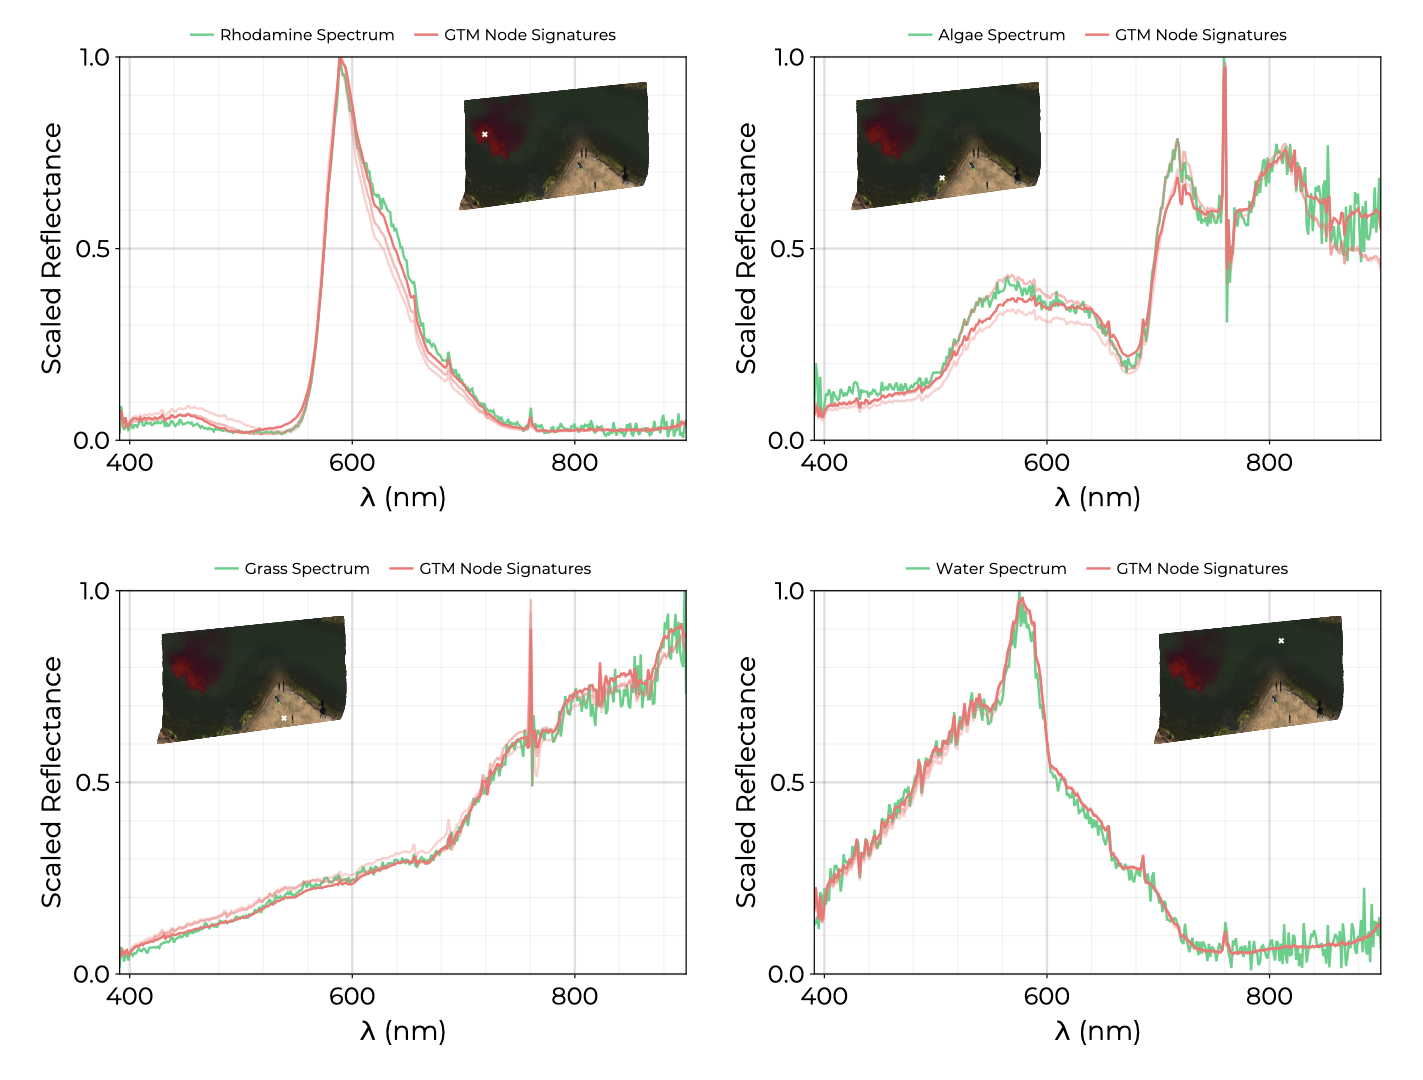
\includegraphics[width=15.5cm]{paper/figures/results/spectral-signatures.png}
\end{adjustwidth}
\caption{GTM Node Signatures corresponding to the exemplar spectra for the rhodamine plume (top left), algae (top right), dry grass (bottom left), and open water (bottom right). \label{fig:spectral-signautes}}
\end{figure}  

\subsection{Water Class Map}

\begin{figure}[t]
\begin{adjustwidth}{-\extralength}{0cm}
\centering
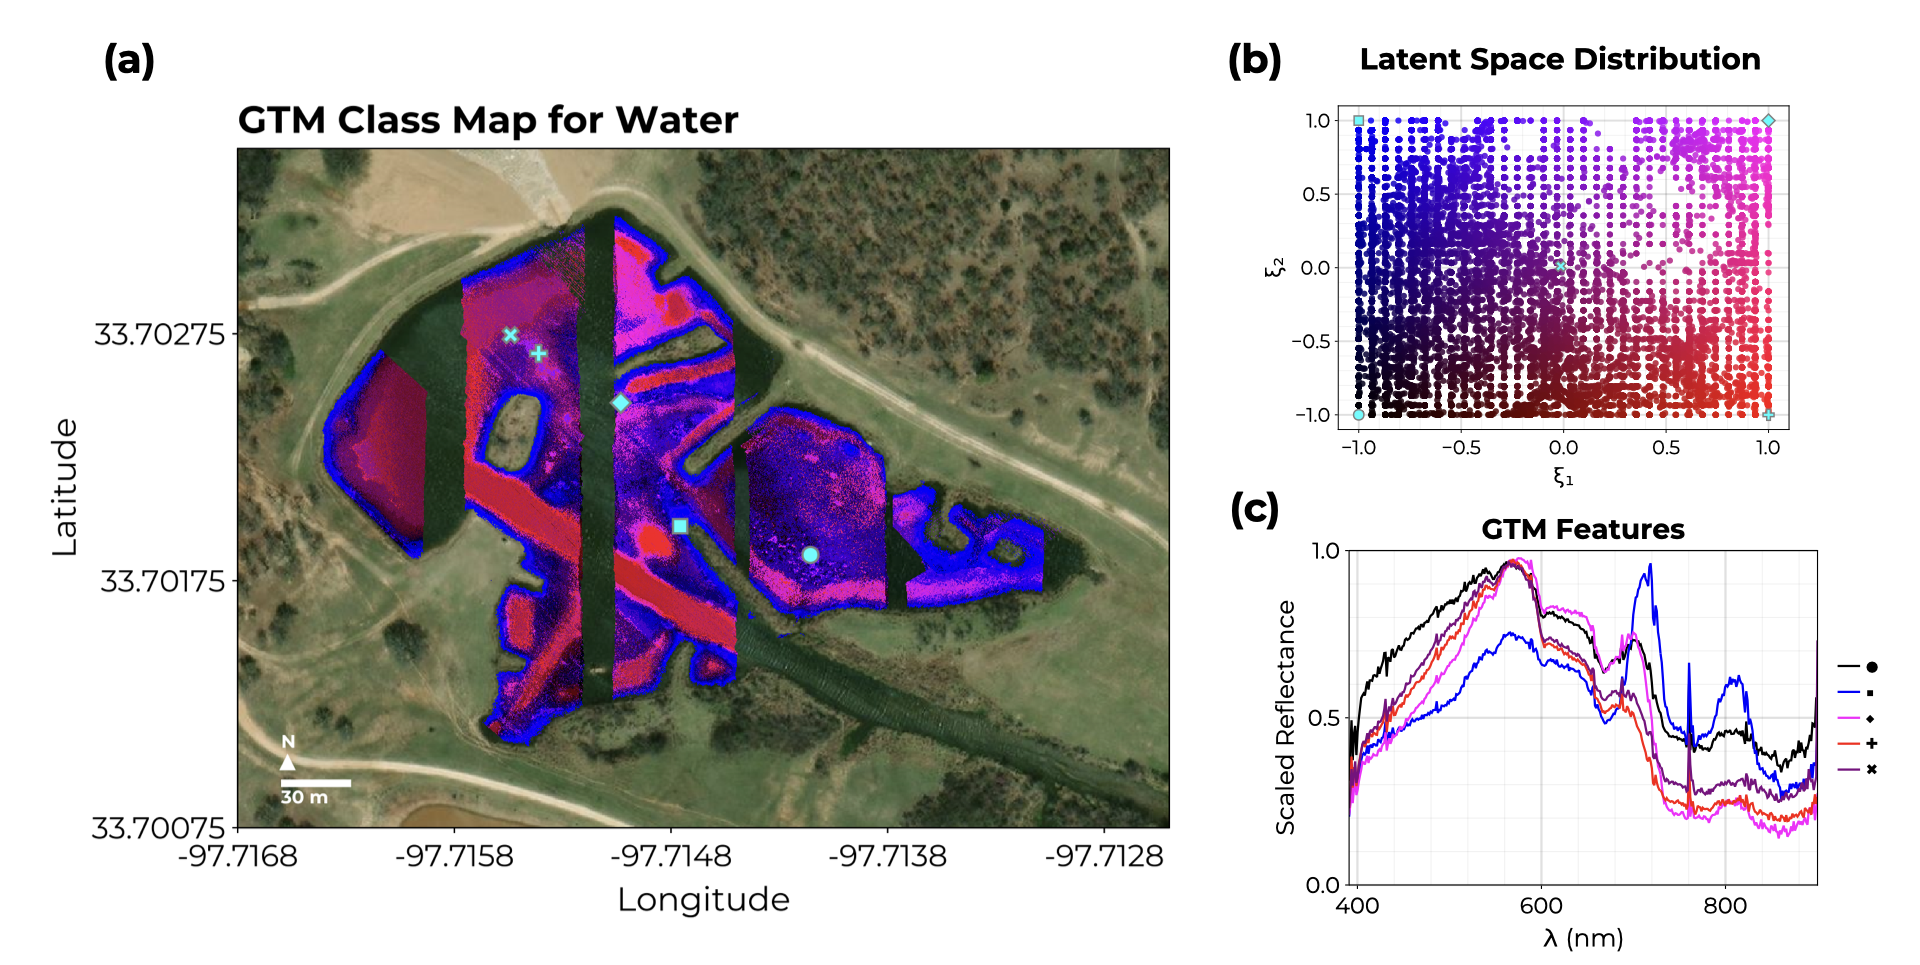
\includegraphics[width=18.0cm]{paper/figures/results/gtm-water.png}
\end{adjustwidth}
\caption{Classification map for GTM trained solely on water pixels (no land and no rhodamine plume). \textbf{(a)} GTM applied to all water pixels colored by their associated position in the latent space. \textbf{(b)} Representation of the poitns from the training set in the latent space. The points are colored with $\xi_1$ corresponding to red and $\xi_2$ corresponding to blue. \textbf{(c)} The associated GTM spectral signatures, $\Psi_i$, corresponding to the four corners and center of the GTM latent space. \label{fig:gtm-water}}
\end{figure}  


\subsection{Algae Identification}


\begin{figure}[t]
\begin{adjustwidth}{-\extralength}{0cm}
\centering
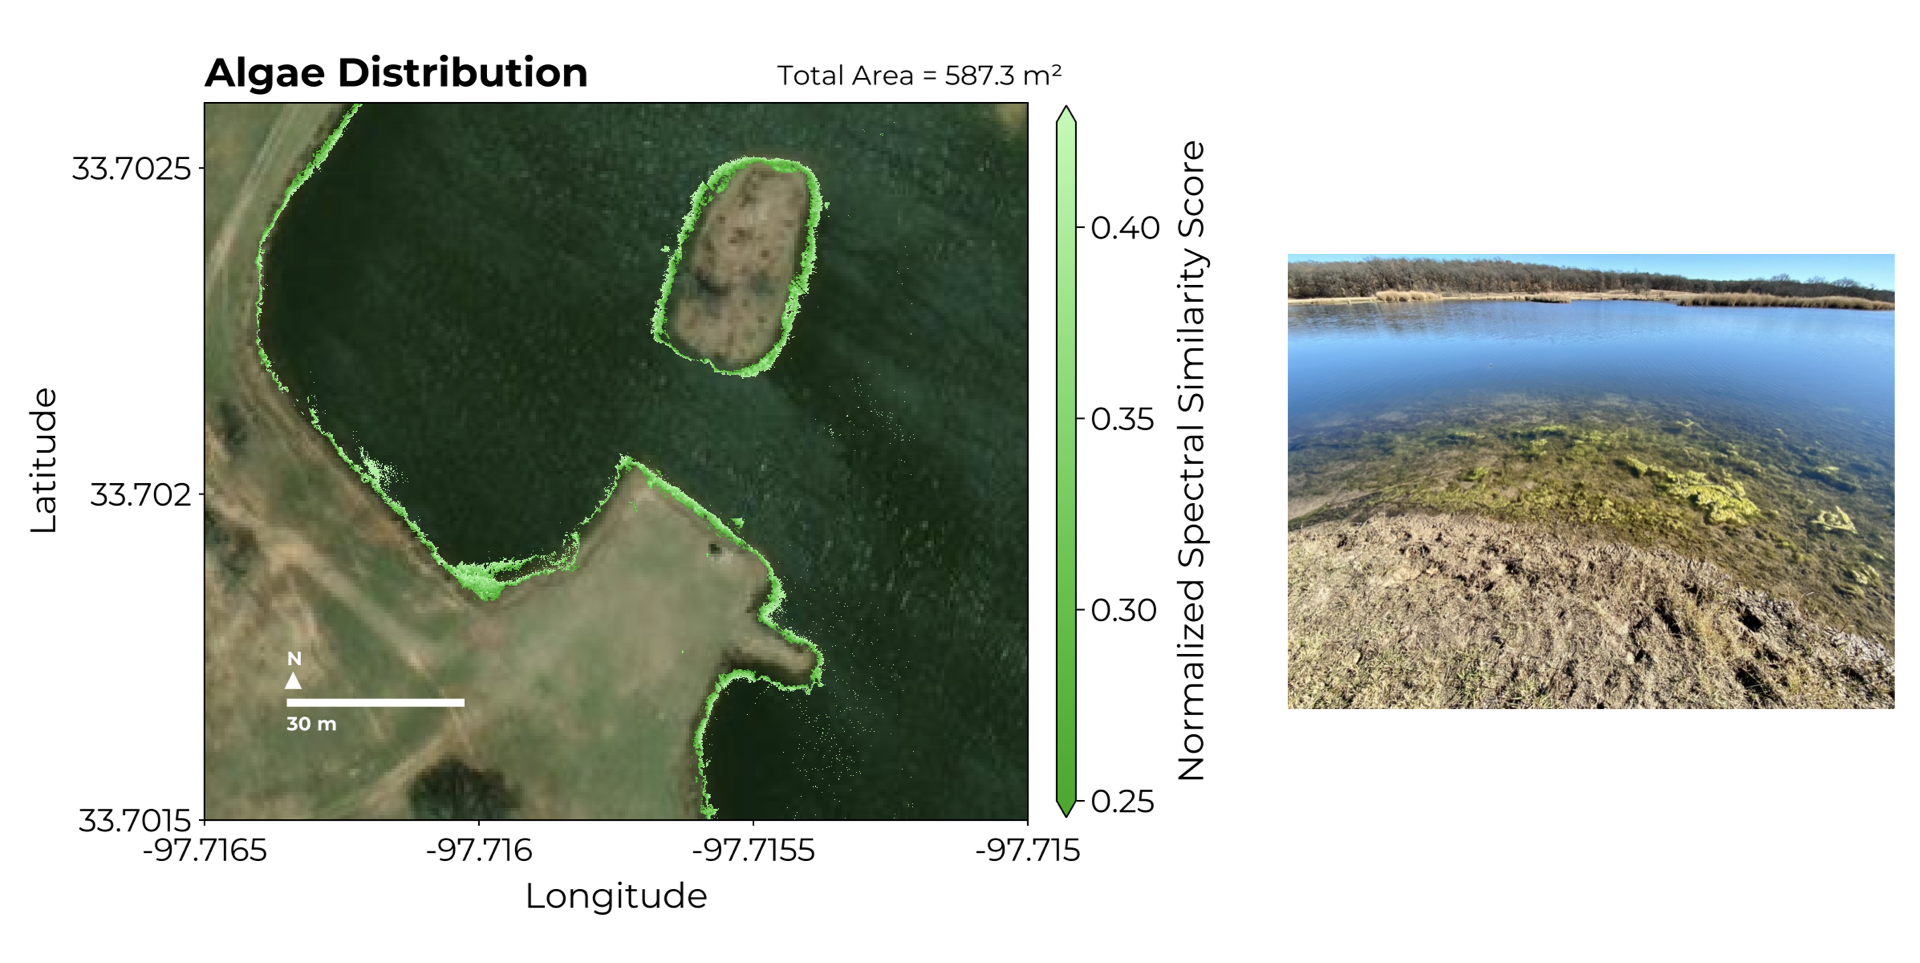
\includegraphics[width=15.5cm]{paper/figures/results/algae.png}
\end{adjustwidth}
\caption{\label{fig:algae-map}}
\end{figure}  



\subsection{Rhodamine Dye Plume Identification}

\begin{figure}[t]
\begin{adjustwidth}{-\extralength}{0cm}
\centering
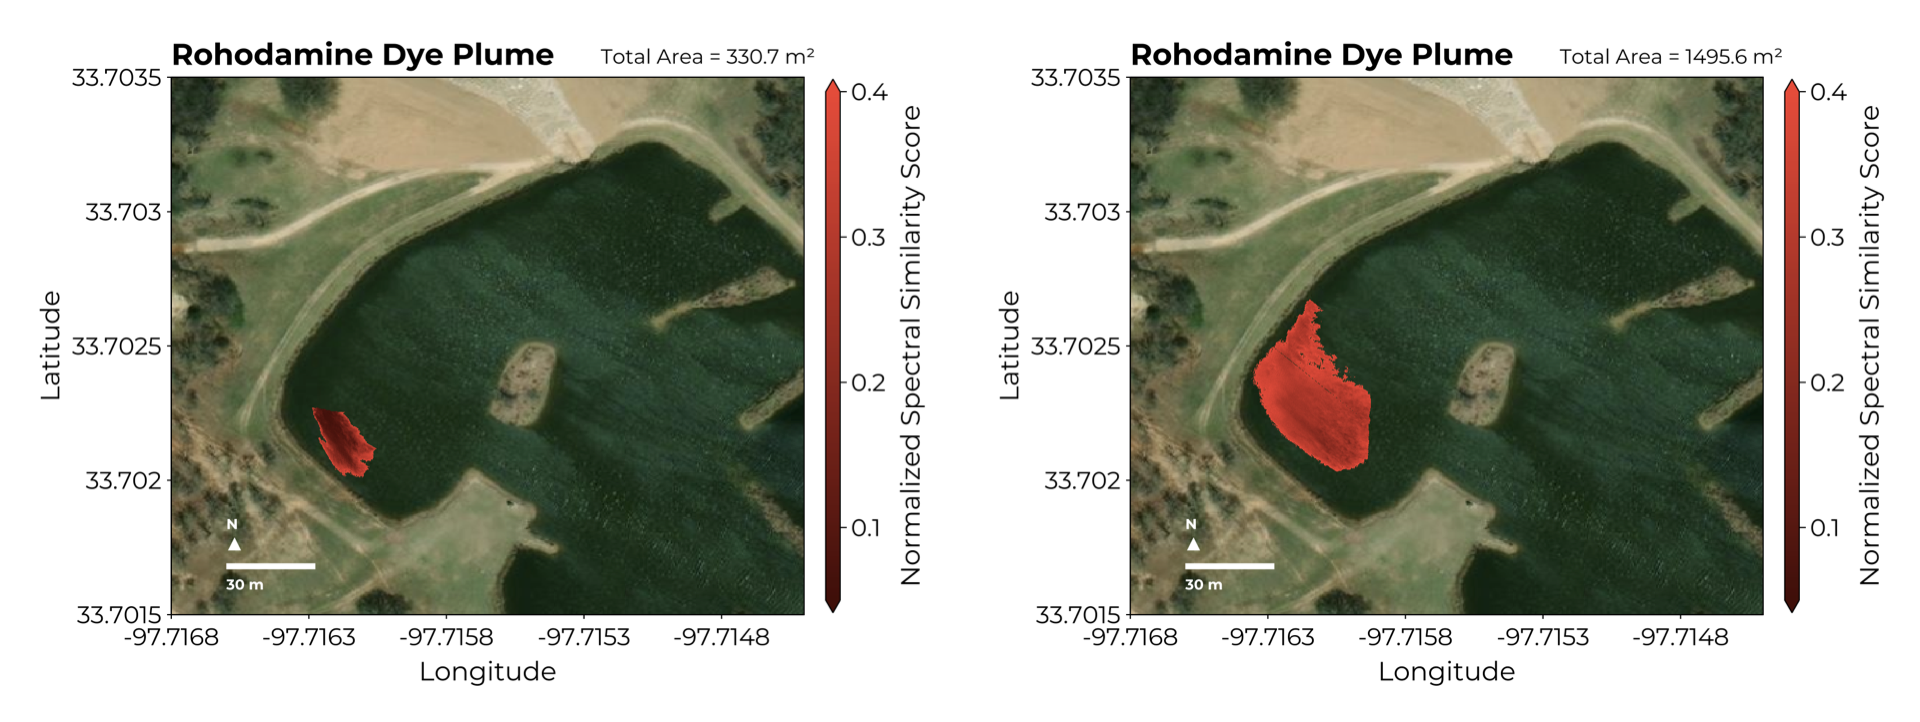
\includegraphics[width=15.5cm]{paper/figures/results/rhodamine.png}
\end{adjustwidth}
\caption{\label{fig:rhodamine-map}}
\end{figure}  




%%%%%%%%%%%%%%%%%%%%%%%%%%%%%%%%%%%%%%%%%%
\section{Discussion}

\subsection{Summary of GTM applications in our paper}
\subsection{Comparison to other existing approaches in literature}
- Is there much done for classification in real time? 
\subsection{Comparison to Spectral Unmixing}
- Here we can re-interpret the GTM model as performing a type of Bayesian spectral unmixing and suggest how the method could be further extended to work in this domain. Critically, other traditional methods work by observing that pure endmembers form the vertices of a simplex. 

\subsection{Other applications of GTM}
- Discuss use of GTM means/modes/responsibilities feature transformer for supervised models (e.g. better than PCA) 
- Use of GTM classes to aid autonomous data collection by identification of "interesting" regons


%%%%%%%%%%%%%%%%%%%%%%%%%%%%%%%%%%%%%%%%%%
\section{Conclusions}


%%%%%%%%%%%%%%%%%%%%%%%%%%%%%%%%%%%%%%%%%%
\vspace{6pt} 

%%%%%%%%%%%%%%%%%%%%%%%%%%%%%%%%%%%%%%%%%%
%% optional
%\supplementary{The following supporting information can be downloaded at:  \linksupplementary{s1}, Figure S1: title; Table S1: title; Video S1: title.}

% Only for journal Methods and Protocols:
% If you wish to submit a video article, please do so with any other supplementary material.
% \supplementary{The following supporting information can be downloaded at: \linksupplementary{s1}, Figure S1: title; Table S1: title; Video S1: title. A supporting video article is available at doi: link.}

% Only for journal Hardware:
% If you wish to submit a video article, please do so with any other supplementary material.
% \supplementary{The following supporting information can be downloaded at: \linksupplementary{s1}, Figure S1: title; Table S1: title; Video S1: title.\vspace{6pt}\\
%\begin{tabularx}{\textwidth}{lll}
%\toprule
%\textbf{Name} & \textbf{Type} & \textbf{Description} \\
%\midrule
%S1 & Python script (.py) & Script of python source code used in XX \\
%S2 & Text (.txt) & Script of modelling code used to make Figure X \\
%S3 & Text (.txt) & Raw data from experiment X \\
%S4 & Video (.mp4) & Video demonstrating the hardware in use \\
%... & ... & ... \\
%\bottomrule
%\end{tabularx}
%}

%%%%%%%%%%%%%%%%%%%%%%%%%%%%%%%%%%%%%%%%%%
\authorcontributions{FIXME}

\funding{FIXME}

\institutionalreview{Not applicable}

\informedconsent{Not applicable}

\dataavailability{We encourage all authors of articles published in MDPI journals to share their research data. In this section, please provide details regarding where data supporting reported results can be found, including links to publicly archived datasets analyzed or generated during the study. Where no new data were created, or where data is unavailable due to privacy or ethical restrictions, a statement is still required. Suggested Data Availability Statements are available in section ``MDPI Research Data Policies'' at \url{https://www.mdpi.com/ethics}.} 


\acknowledgments{In this section you can acknowledge any support given which is not covered by the author contribution or funding sections. This may include administrative and technical support, or donations in kind (e.g., materials used for experiments).}

\conflictsofinterest{Declare conflicts of interest or state ``The authors declare no conflicts of interest.'' Authors must identify and declare any personal circumstances or interest that may be perceived as inappropriately influencing the representation or interpretation of reported research results. Any role of the funders in the design of the study; in the collection, analyses or interpretation of data; in the writing of the manuscript; or in the decision to publish the results must be declared in this section. If there is no role, please state ``The funders had no role in the design of the study; in the collection, analyses, or interpretation of data; in the writing of the manuscript; or in the decision to publish the results''.} 

%%%%%%%%%%%%%%%%%%%%%%%%%%%%%%%%%%%%%%%%%%
%% Optional

%% Only for journal Encyclopedia
%\entrylink{The Link to this entry published on the encyclopedia platform.}

\abbreviations{Abbreviations}{
The following abbreviations are used in this manuscript:\\

\noindent 
\begin{tabular}{@{}ll}
UAV & Unmanned Aerial Vehicle \\
SOM & Self Organizing Map \\ 
GTM & Generative Topographic Mapping 
HSI & Hyperspectral Image \\ 
CDOM & Colored Dissolved Organic Matter \\
HAB & Harmful Algal Bloom 
\end{tabular}
}

%%%%%%%%%%%%%%%%%%%%%%%%%%%%%%%%%%%%%%%%%%
%% Optional
\appendixtitles{yes} % Leave argument "no" if all appendix headings stay EMPTY (then no dot is printed after "Appendix A"). If the appendix sections contain a heading then change the argument to "yes".
\appendixstart
\appendix
\section[\appendixname~\thesection]{Hyperparameter Search Results}

\begin{table}[H]
  \caption{The top 25 models from the hyperparameter search. A variety of GTM were trained to explore the the impact of varying m, $\alpha$, and s.\label{tab:hp-search}}
  \begin{adjustwidth}{-\extralength}{0cm}
  \newcolumntype{C}{>{\centering\arraybackslash}X}
  \begin{tabularx}{\fulllength}{CCCCCC}
    \toprule
    \textbf{m} & \textbf{$\alpha$} & \textbf{s} & \textbf{k} & \textbf{BIC} & \textbf{AIC} \\
    \midrule
    14 & 0.1 & 1.0 & 32 & \textbf{-1.918e8} & -1.926e8\\
    13 & 0.01 & 1.0 & 32 & -1.917e8 & -1.923e8\\
    16 & 0.01 & 1.5 & 32 & -1.917e8 & -1.926e8\\
    14 & 10.0 & 1.0 & 32 & -1.917e8 & -1.924e8\\
    16 & 0.001 & 1.5 & 32 & -1.917e8 & -1.926e8\\
    13 & 1.0 & 1.0 & 32 & -1.917e8 & -1.923e8\\
    13 & 10.0 & 1.0 & 32 & -1.917e8 & -1.923e8\\
    14 & 0.001 & 1.5 & 32 & -1.916e8 & -1.924e8\\
    13 & 0.1 & 1.0 & 32 & -1.916e8 & -1.923e8\\
    14 & 0.01 & 1.0 & 32 & -1.916e8 & -1.924e8\\
    15 & 0.01 & 1.5 & 32 & -1.916e8 & -1.925e8\\
    14 & 0.01 & 1.5 & 32 & -1.916e8 & -1.923e8\\
    15 & 1.0 & 1.0 & 32 & -1.916e8 & -1.924e8\\
    18 & 0.01 & 1.5 & 32 & -1.916e8 & -1.928e8\\
    12 & 0.01 & 1.0 & 32 & -1.916e8 & -1.921e8\\
    15 & 0.01 & 0.5 & 32 & -1.915e8 & -1.924e8\\
    17 & 1.0 & 1.0 & 32 & -1.915e8 & -1.926e8\\
    16 & 0.1 & 1.0 & 32 & -1.915e8 & -1.925e8\\
    18 & 0.001 & 1.5 & 32 & -1.915e8 & -1.928e8\\
    13 & 0.001 & 1.0 & 32 & -1.915e8 & -1.922e8\\
    12 & 1.0 & 1.0 & 32 & -1.915e8 & -1.921e8\\
    17 & 0.001 & 1.5 & 32 & -1.915e8 & -1.926e8\\
    15 & 0.001 & 1.5 & 32 & -1.915e8 & -1.923e8\\
    15 & 10.0 & 1.0 & 32 & -1.915e8 & -1.923e8\\
    12 & 0.1 & 1.5 & 32 & -1.915e8 & -1.92e8\\
    \bottomrule
  \end{tabularx}
  \end{adjustwidth}
\end{table}


%%%%%%%%%%%%%%%%%%%%%%%%%%%%%%%%%%%%%%%%%%
\begin{adjustwidth}{-\extralength}{0cm}
%\printendnotes[custom] % Un-comment to print a list of endnotes

\reftitle{References}

%=====================================
% References, variant A: external bibliography
%=====================================
\bibliography{paper/references.bib}

%%%%%%%%%%%%%%%%%%%%%%%%%%%%%%%%%%%%%%%%%%
\PublishersNote{}
\end{adjustwidth}
\end{document}

